\begin{figure}[!ht]
	\centering
	\subfigure[][Appearance changes]{\label{fig:changes}
	    \begin{minipage}[b]{0.45\linewidth}
   			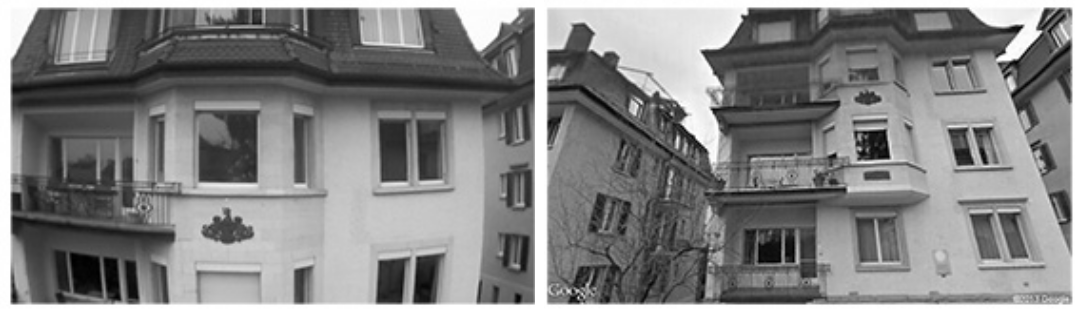
\includegraphics[width=\linewidth]{changes/viewpoint.png}

			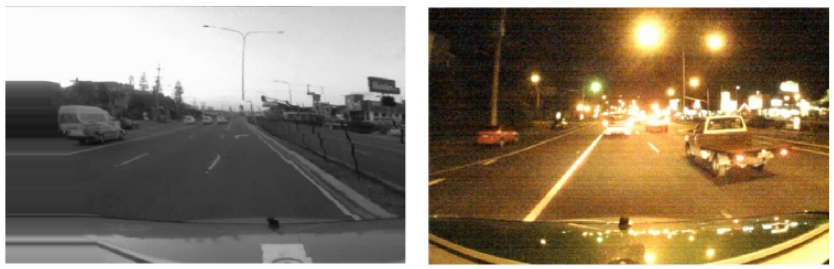
\includegraphics[width=\linewidth]{changes/daynight.png}

			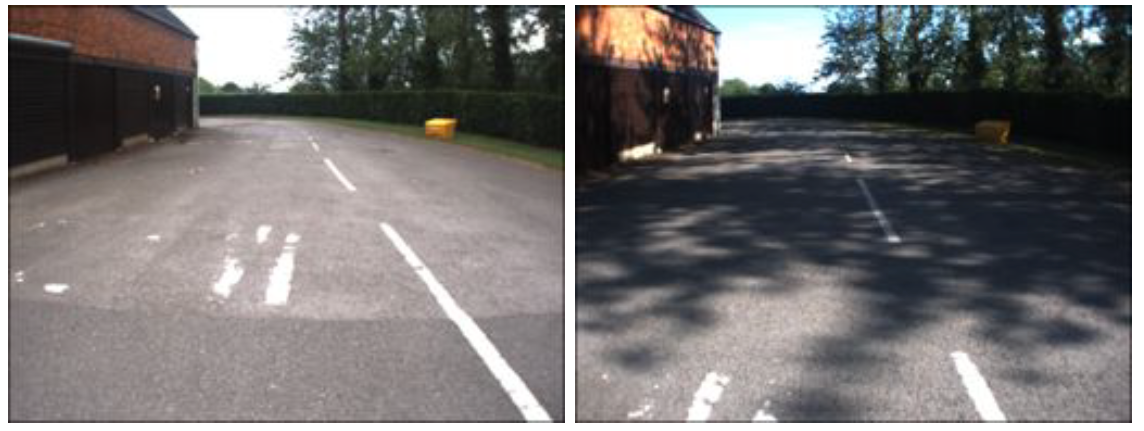
\includegraphics[width=\linewidth]{changes/shadow.png}
	    \end{minipage}
	}
	\begin{minipage}[b]{0.53\linewidth}
   		\subfigure[][Cross-view]{\label{fig:cross-view}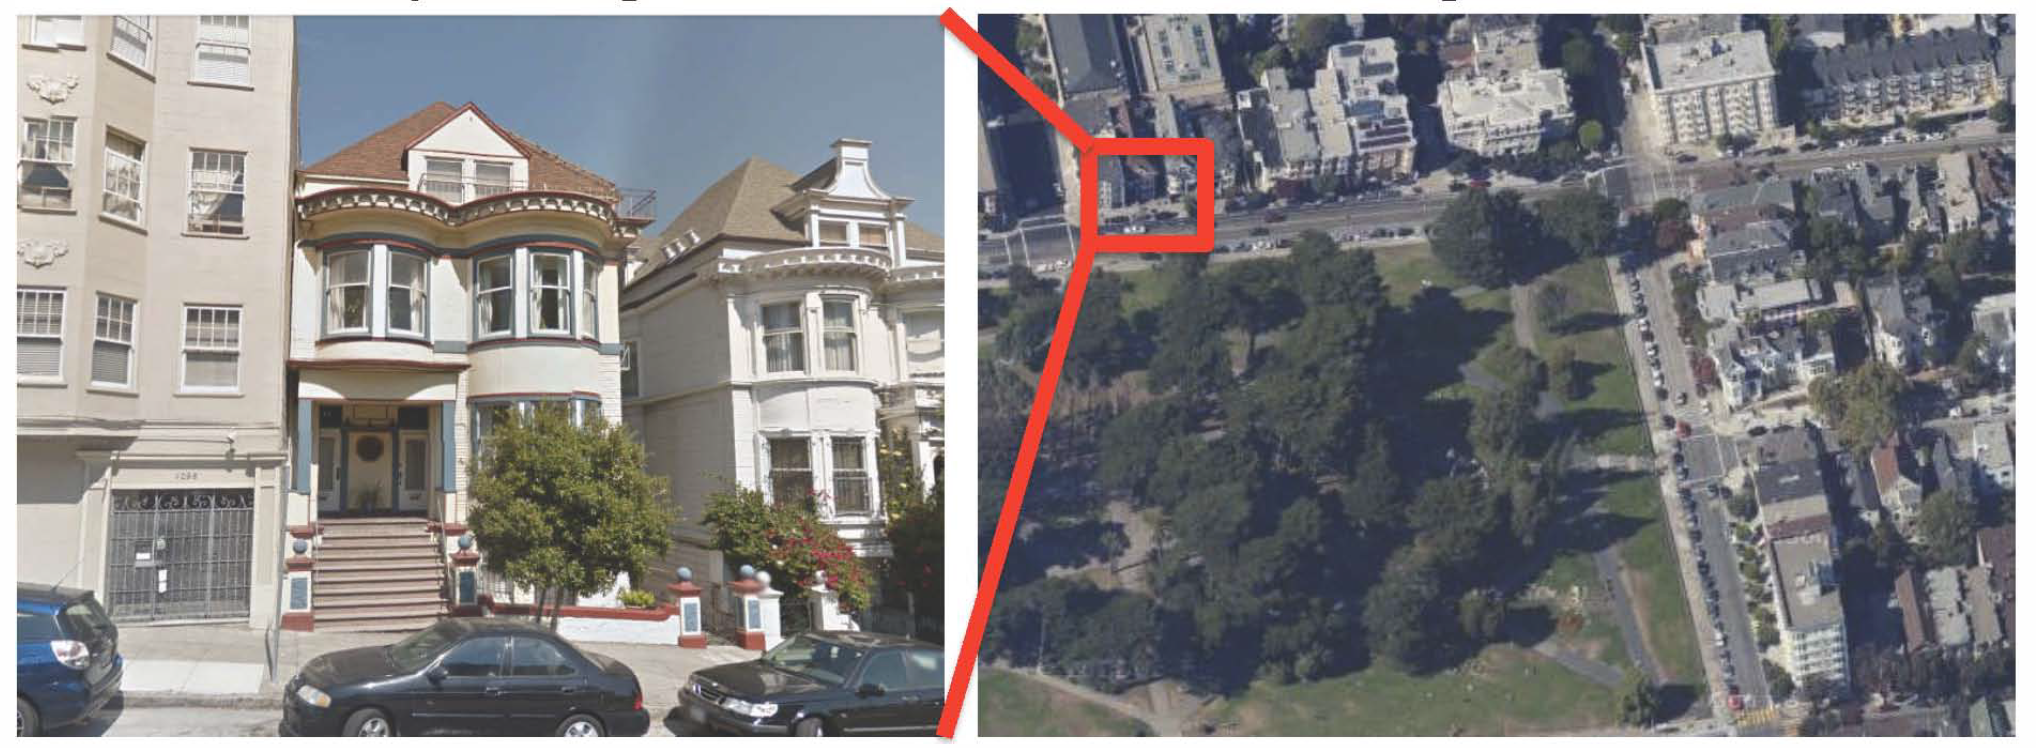
\includegraphics[width=\linewidth]{changes/cross-view.png}}
   		    
   		\subfigure[][Cross-domain]{\label{fig:cross-domain}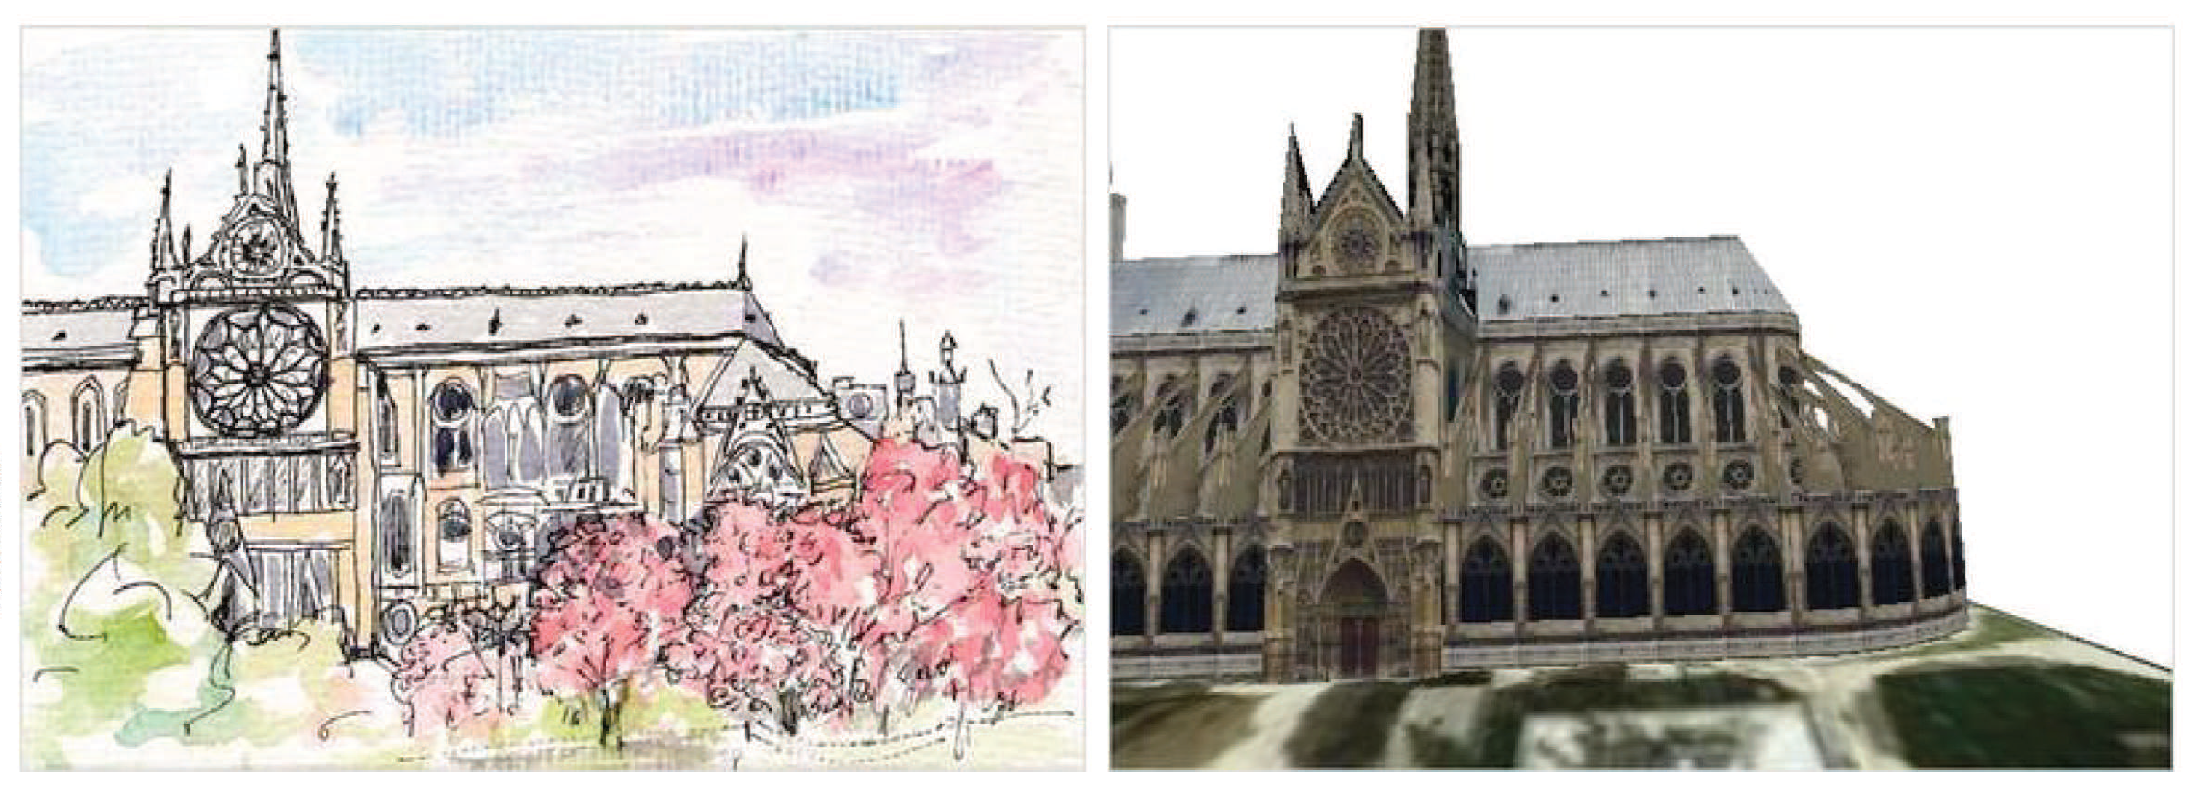
\includegraphics[width=\linewidth]{changes/cross-domain.png}}
	\end{minipage}
	\caption[Illustration of appearance changes present in \ac{vbl} system]{\textbf{Illustration of appearance changes present in \ac{vbl} system:} \ref{fig:changes}~Visual dissimilarity between the query (left) and the closest image in the database (right). Cause of the change, from top to bottom:~viewpoint differences in a system for MAV localization in urban environment from \citep{Majdik2013}, extreme illumination changes from \citep{Milford2015}, shadow interferences from \citep{Corke2013}. \ref{fig:cross-view}~Cross-view localization system from \citep{Lin2015}:~left represent the ground-level query image and right the bird's eye view of the same scene (red rectangle). \ref{fig:cross-domain}~Cross-domain \ac{vbl} system from \citep{Aubry2014}:~on the left the query painting and on the right the corresponding pose according to a 3D model. \label{fig:data_changes}}
\end{figure}
